% =====================================================================
% Dissertation Proposal -- Presentation slides (Beamer)
% Lineage-Aware Hierarchical Deep Learning for Imbalanced Multi-Class
% Classification of Peripheral Blood Cells
%
% Needs the figure files in the same folder:
%   cell_category.pdf   (two-level lineage hierarchy)
%   Methodology-1.pdf   (methodology pipeline)
%
% Compile with: pdflatex Proposal_Slides.tex  (run twice)
% =====================================================================
\documentclass[aspectratio=169,11pt]{beamer}

\usepackage{graphicx}
\graphicspath{{../assets/}{../../artifacts/}{./}}
\usetheme{Madrid}
\usecolortheme{default}
\setbeamertemplate{navigation symbols}{}
\setbeamertemplate{caption}[numbered]
\setbeamercovered{transparent}
\setbeamertemplate{itemize items}[circle]

\title[Hierarchical Blood-Cell Classification]{Lineage-Aware Hierarchical Deep Learning for
Imbalanced Multi-Class Classification of Peripheral Blood Cells}
\subtitle{Dissertation Proposal}
\author{Arthiga Karthigesu}
\date{}

\begin{document}

% ---------------------------------------------------------------- Slide 1
\begin{frame}[plain]
  \titlepage
\end{frame}

% ---------------------------------------------------------------- Slide 2
\begin{frame}{Background and the problem}
  \begin{itemize}
    \item Reading a blood smear is a core step in diagnosing blood diseases,
          including leukaemia.
    \item An expert labels each cell by its shape, chromatin, cytoplasm, and
          granularity.
    \item This manual count is slow and repetitive. It also varies between
          observers.
    \item It is hardest for rare and immature cells, whose look overlaps with
          neighbouring types.
    \item Deep models already match experts on some tasks (Matek et al., 2019).
  \end{itemize}

  \vspace{0.4em}
  \begin{alertblock}{The problem}
    Most systems treat all 18 cell types as flat, unrelated labels. They ignore
    the biology. The data is also highly imbalanced, so rare cells are easily
    missed.
  \end{alertblock}
\end{frame}

% ---------------------------------------------------------------- Slide 3
\begin{frame}{Research gap and research question}
  Four research lines are strong on their own, but they have not been combined:
  \begin{itemize}
    \item Deep models for blood-cell images.
    \item Hierarchical classification that uses label structure.
    \item Loss functions that are robust to class imbalance.
    \item Explainable models, such as Grad-CAM.
  \end{itemize}

  \begin{block}{Research gap}
    No study so far brings together a biology-based lineage hierarchy, an
    imbalance-robust loss, and saliency checks on a single, highly imbalanced
    blood dataset.
  \end{block}

  \begin{exampleblock}{Research question}
    Does a lineage-aware hierarchical classifier, with an imbalance-robust loss,
    improve fine-grained classification, and especially the rare cell types,
    compared with a flat classifier on the same data?
  \end{exampleblock}
\end{frame}

% ---------------------------------------------------------------- Slide 4
\begin{frame}{Methodology}
  \begin{columns}[T]
    \begin{column}{0.5\textwidth}
      \textbf{Data}
      \begin{itemize}
        \item MLL23 dataset: 41,621 single-cell images, 18 classes.
        \item About a 260-fold gap between the largest and smallest class.
        \item Two-level label hierarchy: lineage first, then fine cell type.
      \end{itemize}
      \vspace{0.3em}
      \textbf{Model}
      \begin{itemize}
        \item Shared transfer-learning backbone.
        \item Backbones to compare: MobileNet, ResNet, ConvNeXt, and a Vision
              Transformer.
        \item Two heads: one for lineage, one for fine type.
        \item Class-balanced hierarchical loss for rare classes.
      \end{itemize}
    \end{column}
    \begin{column}{0.5\textwidth}
      \textbf{Training and evaluation}
      \begin{itemize}
        \item Stratified split, so rare classes appear in every set.
        \item Stronger augmentation on minority classes.
        \item Compare against a flat baseline.
        \item Ablation: remove the loss term, then the hierarchy.
        \item Metrics: macro F1, balanced accuracy, confusion matrix.
        \item Grad-CAM for visual explanations.
      \end{itemize}
    \end{column}
  \end{columns}
\end{frame}

% ---------------------------------------------------------------- Slide 5
\begin{frame}{Two-level lineage hierarchy}
  \centering
  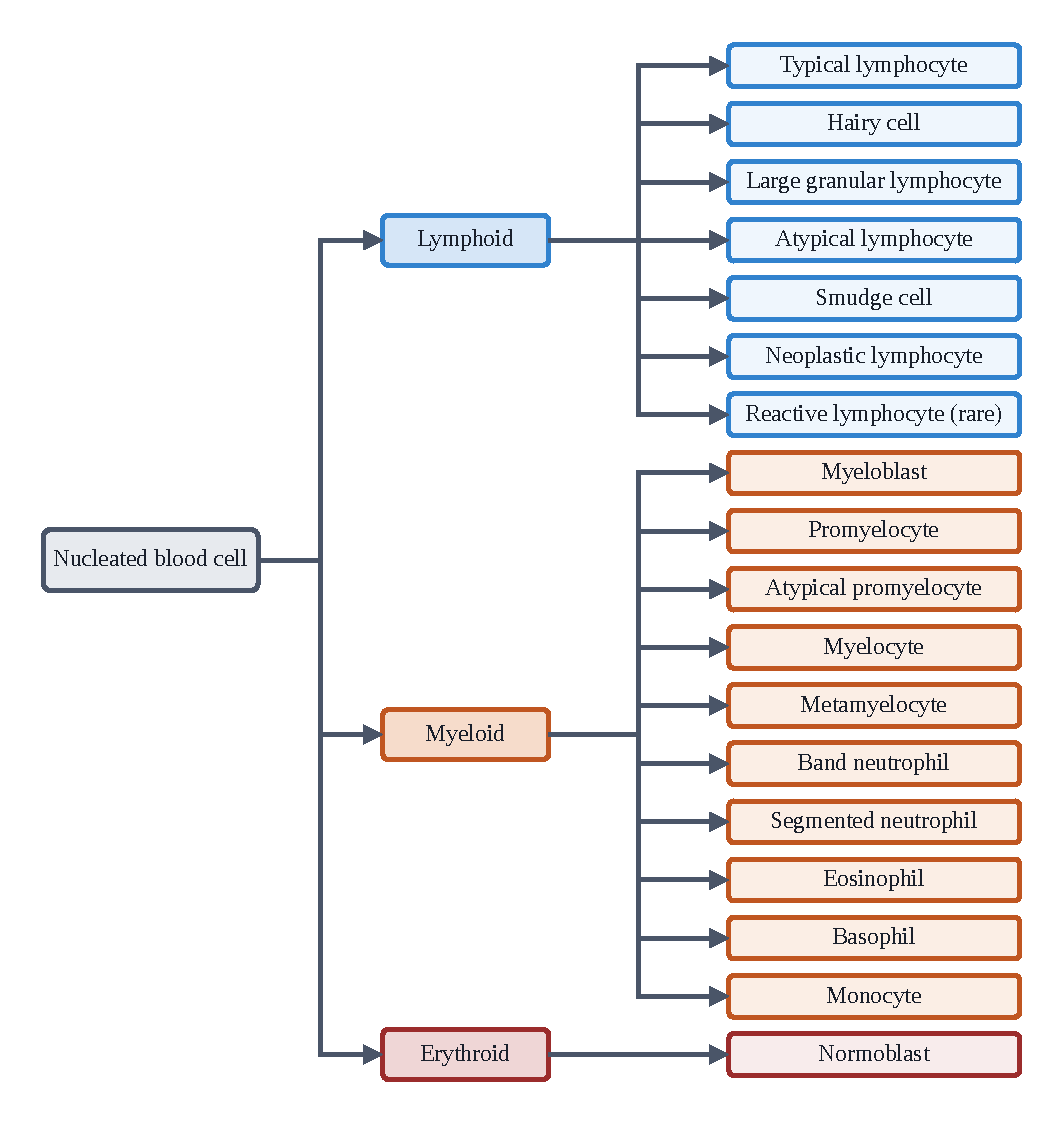
\includegraphics[height=0.80\textheight]{cell_category.pdf}
\end{frame}

% ---------------------------------------------------------------- Slide 6
\begin{frame}{Proposed pipeline}
  \centering
  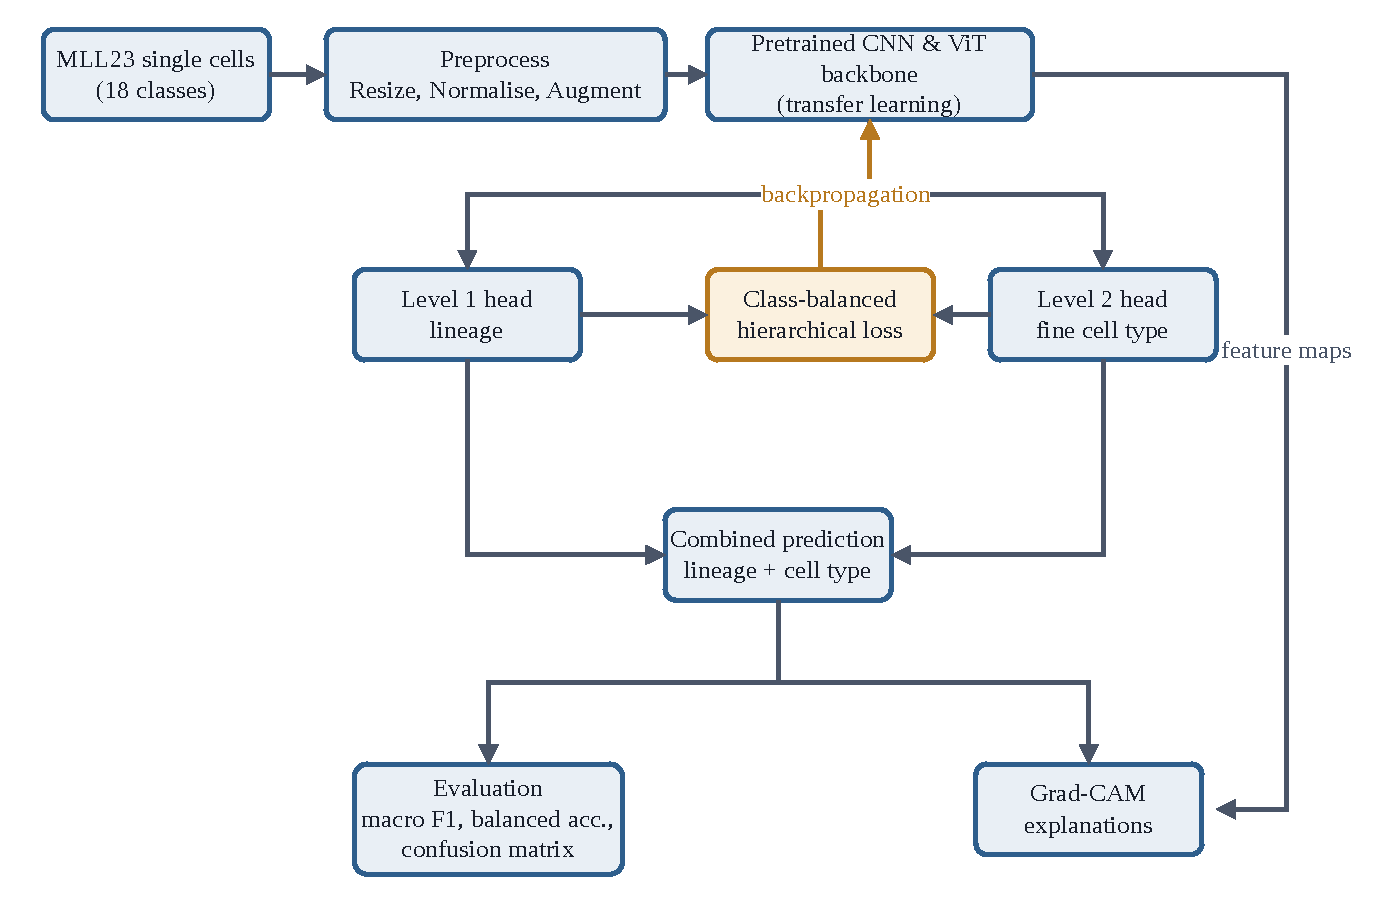
\includegraphics[width=0.79\textwidth]{Methodology-1.pdf}

  \vspace{0.5em}
  {\footnotesize During training, the class-balanced hierarchical loss updates the
  backbone. At inference, the combined prediction is evaluated and explained with
  Grad-CAM.}
\end{frame}

% ---------------------------------------------------------------- Slide 7
\begin{frame}{Expected outcomes}
  \begin{itemize}
    \item Higher macro F1 and balanced accuracy than the flat baseline.
    \item The largest gains on the rare cell types.
    \item Fewer errors that cross unrelated lineages.
    \item Ablation shows what the hierarchy and the loss each add.
    \item Grad-CAM confirms the model looks at meaningful regions, such as the
          nucleus, the chromatin, and the cytoplasm.
    \item A reusable, interpretable pipeline for imbalanced single-cell
          classification.
  \end{itemize}
\end{frame}

% ---------------------------------------------------------------- Slide 8
\begin{frame}{Summary}
  \begin{itemize}
    \item The model is shaped by blood-cell biology, not by flat labels.
    \item It joins a lineage hierarchy, an imbalance-robust loss, and saliency
          checks in one pipeline.
    \item It is tested on the largest public single-cell blood dataset.
    \item The focus is the rare cells that matter most in the clinic.
  \end{itemize}

  \vspace{1em}
  \begin{center}
    \large Thank you. Questions are welcome.
  \end{center}
\end{frame}

\end{document}
